\hypertarget{ux7535ux5b50ux90aeux4ef6}{%
\subsection{电子邮件}\label{ux7535ux5b50ux90aeux4ef6}}

Email 的历史比 Web 还要久远,直到现在,Email
也是互联网上应用非常广泛的服务。

几乎所有的编程语言都支持发送和接收电子邮件,但是,先等等,在我们开始编写代码之前,有必要搞清楚电子邮件是如何在互联网上运作的。

我们来看看传统邮件是如何运作的。假设你现在在北京,要给一个香港的朋友发一封信,怎么做呢?

首先你得写好信,装进信封,写上地址,贴上邮票,然后就近找个邮局,把信仍进去。

信件会从就近的小邮局转运到大邮局,再从大邮局往别的城市发,比如先发到天津,再走海运到达香港,也可能走京九线到香港,但是你不用关心具体路线,你只需要知道一件事,就是信件走得很慢,至少要几天时间。

信件到达香港的某个邮局,也不会直接送到朋友的家里,因为邮局的叔叔是很聪明的,他怕你的朋友不在家,一趟一趟地白跑,所以,信件会投递到你的朋友的邮箱里,邮箱可能在公寓的一层,或者家门口,直到你的朋友回家的时候检查邮箱,发现信件后,就可以取到邮件了。

电子邮件的流程基本上也是按上面的方式运作的,只不过速度不是按天算,而是按秒算。

现在我们回到电子邮件,假设我们自己的电子邮件地址是\texttt{me@163.com},对方的电子邮件地址是\texttt{friend@sina.com}(注意地址都是虚构的哈),现在我们用\texttt{Outlook}或者\texttt{Foxmail}之类的软件写好邮件,填上对方的
Email 地址,点 ``发送'',电子邮件就发出去了。这些电子邮件软件被称为
\textbf{MUA}:Mail User Agent------邮件用户代理。

Email 从 MUA 发出去,不是直接到达对方电脑,而是发到 \textbf{MTA}:Mail
Transfer Agent------邮件传输代理,就是那些 Email
服务提供商,比如网易、新浪等等。由于我们自己的电子邮件是\texttt{163.com},所以,Email
首先被投递到网易提供的 MTA,再由网易的 MTA 发到对方服务商,也就是新浪的
MTA。这个过程中间可能还会经过别的
MTA,但是我们不关心具体路线,我们只关心速度。

Email 到达新浪的 MTA
后,由于对方使用的是\texttt{@sina.com}的邮箱,因此,新浪的 MTA 会把
Email 投递到邮件的最终目的地 \textbf{MDA}:Mail Delivery
Agent------邮件投递代理。Email 到达 MDA
后,就静静地躺在新浪的某个服务器上,存放在某个文件或特殊的数据库里,我们将这个长期保存邮件的地方称之为电子邮箱。

同普通邮件类似,Email
不会直接到达对方的电脑,因为对方电脑不一定开机,开机也不一定联网。对方要取到邮件,必须通过
MUA 从 MDA 上把邮件取到自己的电脑上。

所以,一封电子邮件的旅程就是:

\begin{pythoncode}
发件人 -> MUA -> MTA -> MTA -> 若干个MTA -> MDA <- MUA <- 收件人
\end{pythoncode}

有了上述基本概念,要编写程序来发送和接收邮件,本质上就是:

\begin{enumerate}
\def\labelenumi{\arabic{enumi}.}
\item
  编写 MUA 把邮件发到 MTA;
\item
  编写 MUA 从 MDA 上收邮件。
\end{enumerate}

发邮件时,MUA 和 MTA 使用的协议就是 SMTP:Simple Mail Transfer
Protocol,后面的 MTA 到另一个 MTA 也是用 SMTP 协议。

收邮件时,MUA 和 MDA 使用的协议有两种:POP:Post Office
Protocol,目前版本是 3,俗称 POP3;IMAP:Internet Message Access
Protocol,目前版本是 4,优点是不但能取邮件,还可以直接操作 MDA
上存储的邮件,比如从收件箱移到垃圾箱,等等。

邮件客户端软件在发邮件时,会让你先配置 SMTP 服务器,也就是你要发到哪个
MTA 上。假设你正在使用 163 的邮箱,你就不能直接发到新浪的 MTA
上,因为它只服务新浪的用户,所以,你得填 163 提供的 SMTP
服务器地址:\texttt{smtp.163.com},为了证明你是 163 的用户,SMTP
服务器还要求你填写邮箱地址和邮箱口令,这样,MUA 才能正常地把 Email 通过
SMTP 协议发送到 MTA。

类似的,从 MDA 收邮件时,MDA
服务器也要求验证你的邮箱口令,确保不会有人冒充你收取你的邮件,所以,Outlook
之类的邮件客户端会要求你填写 POP3 或 IMAP
服务器地址、邮箱地址和口令,这样,MUA 才能顺利地通过 POP 或 IMAP 协议从
MDA 取到邮件。

在使用 Python
收发邮件前,请先准备好至少两个电子邮件,如\texttt{xxx@163.com},\texttt{xxx@sina.com},\texttt{xxx@qq.com}等,注意两个邮箱不要用同一家邮件服务商。

最后\_特别注意\_,目前大多数邮件服务商都需要手动打开 SMTP 发信和 POP
收信的功能,否则只允许在网页登录:

 
 \begin{figure}[htp]
	\centering
	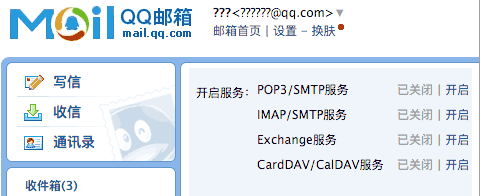
\includegraphics[width=0.6\linewidth]{fig/1050933742009056l.png}
\end{figure}


